\documentclass{article}
\usepackage[utf8]{inputenc}
\usepackage{custom}

\title{INMA 2361 - Nonlinear dynamical systems \\
        Project : Language dynamics}
\author{Quentin Lété}
\date{January 2018}

\begin{document}

\maketitle

\section{Introduction}
Languages death is a major cultural issue on our planet.
On the aprroximately 7,000 languages in the world, more than half of them are endangered.
It is estimated that one language is dying every two weeks.
90 \% of the languages are expected to disappear with the current generation \cite{death}.
In this context, it is important to come up with models to explain this death so that policies can be adapted.
Many models focused on the properties of the languages like grammar or syntax were developed.
Here we restrict ourselves to the mathematical models in the framework of dynamical systems. \\
Abrams and Strogatz explained in \cite{death} how the death of a language competing with another can be explained with a very simple model.
Other authors (\cite{bilingual}) have extended this model to account for the possibility of bilinguism among the population. In particular, they show when coexistence is possible.
In this work, I propose to extend the two previous models to model the temporal change on the perception of a language when it is endangered.
I will also analyse numerically some spatial properties of the dynamics and test on a real dataset for the Irish case.
As the model developed here is a direct extension of \cite{bilingual} and as a comprehensive state space analysis was made in that paper,
I will in each section recall and explain the important results found in \cite{bilingual} before extending to the new temporal and spatial considerations. \\
This project will be a mix between theoretical results and numerical simulations and is not meant to be comprehensive. Sometimes, intuition will be given using numerical simulations only. \\
The report will be organised as follows : in section \ref{sec:basic},
I will prensent the equations of the models proposed by \cite{death} and \cite{bilingual} and define the notations used.
Section \ref{sec:1d} will describe the extension of the model proposed for the change in the perceived status of a language and apply it to extend the Abrams-Strogatz model.
Section \ref{sec:2d} will do the same for \cite{bilingual}.
Section \ref{sec:spatial} will analyse some spatial properties of the system.
Section \ref{sec:conclusion} will be the conclusion of this project.

\section{Basic models and notations}
\label{sec:basic}
We consider a system of two competing languages X and Y.
Abrams and Strogatz made the assumption that the attractiveness of a language depends on two things : its number of speakers and its perceived status.
The perceived relative status, denoted by $s \in [0;1]$ is the perceived social or economical advantage that one has when one speaks this language.
We denote by $x$ and $y$ the normailized population of speakers of language X and Y, i.e. $x+y=1$. $P_{YX}(x, s)$ is the probability per unit of time that a Y speaker becomes an X speaker. As stated above, it is a function of both $x$ and $s$.
A simple model for the evolution of this system is
\begin{equation}
\label{eq:1dsimple}
\dx = yP_{YX}(x, s) - xP_{XY}(x, s)
\end{equation}
which, as $y = 1-x$, is a 1D system. \\
By interchangability of the two languages, one should have that $P_{XY}(x, s) = P_{YX}(1-x, 1-s)$. Abrams and Strogatz proposed the following function for the probability of switching of language :
\[ P_{YX}(x,s) = cx^as \hspace{1cm} P_{XY}(x,s) = c(1-x)^a(1-s) \]

They empirically determined that the parameter $a$ is quite constant trough many populations, with a mean of $1.31$ on a standard deviation of $0.25$. The parameter $s$ has to be estimated for each separate case. When not explicitly stated, all the simulations of this work will thus be made with $a=1.31$.\\

This model doesn't account for the possibility of existence of a bilingual population.
In some cases, this population plays an important role for the persistence of a language.
A model taking a bilingual population into account was first proposed in \cite{BAGGS19939}.
The idea is to introduce a bilingual population $b$ such that $x+y+b=1$.
They also introduce a parameter $k \in [0;1]$ describing the similarity between the two languages.
If $k = 1$, $Y = X$ whereas if $k = 0$, the languages are totally different.
By simply extending the previous model, we obtain the following equations

\begin{equation}
\label{eq:bil}
\begin{cases}
\dx = yP_{YX} + bP_{BX} - x(P_{XY} + P_{XB}) \\
\dy = xP_{XY} + bP_{BY} - y(P_{YX} + P_{YB}) \\
\db = xP_{XB} + yP_{YB} - b(P_{BX} + P_{BY}) \\
\end{cases}
\end{equation}
with the following transition functions :

\[
\begin{cases}
P_{XB} = c \cdot k (1-s) (1-x)^a \\
P_{YB} = c \cdot k s (1-y)^a \\
P_{BX} = P_{YX} = c \cdot (1-k) s (1-y)^a \\
P_{BY} = P_{XY} = c \cdot (1-k) (1-s) (1-x)^a \\
\end{cases}
\]

This model was validated by the authors who found that it fits correctly the historical data of the evolution of speakers in the case of Galician and Spanish for a value of $k = 0.8$. \\
In \cite{BAGGS19939}, some theoretical results are given about the possibility of coexistence. It is shown that coexistence is indeed possible. In \cite{bilingual}, they are interested in the range of values of $s(k)$ that leads to coexistence. This is done using bifurcation theory. In particular, it is first shown that the system experiences a subcritical Pitchfork bfurcation when $s = \frac{1}{2}$. For the general case $s \ne \frac{1}{2}$, there is also a bifurcation but this time, it is a saddle-node bifurcation. Before a critical value of $k$, the system has one fixed point whereas after, it has three fixed point, one of them being stable. This proves that coexistance is possible.

\section{One dimensional temporal extension}
\label{sec:1d}
In this section, I wish to present an extension of the system (\ref{eq:1dsimple}) to take into account the evolution of the perveiced status $s$.
I extend slightly this notion of status to other factors that can make a person want to learn the language, like the cultural factor.
Indeed, in many cases, the very fact that a regional language is endangered increase its status among the population.
The Irish language is a good example.
When Irish people realised that the possibility of extinction of their language existed, people started to consider it differently.
Policies were established to make the language mandatory at school and it gained a lot of influence so that it became primary to know Irish to be able to be accepted in high ranked colleges or apply to some jobs.
Even closer to us, in Wallonia, one can argue that its decrease in popularity was followed by a small but real increase in its status thanks among other to cultural policies or independent actions.
Moreover, the models described in \cite{death} or \cite{bilingual} aim to help to develop policies.
These policies will often lead to an increase in the status $s$ and it would thus be intereting to have a model where $s$ eveloves dynamically. \\
Modelling this phenomenon can be done by considering a non-stationary $s$. The system (\ref{eq:1dsimple}) would become

\begin{equation}
\label{eq:1dtemp}
\begin{cases}
\dx = c\big( (1-x)sx^a - x(1-s)(1-x)^a \big) \\
\ds = S(x, s) \\
\end{cases}
\end{equation}

where the function $S(x,s)$ will model the dynamics of $s$ and need to be defined.
The requirements for this function are that $S(x,s)$ should be positive when $x$ is small, negative when $x$ is large and $0$ when $s = \frac{1}{2}$.
Moreover, it should be such that $s(t) \in [0;1] \hspace{0.5cm} \forall{t}$.
Finally, it should be anti-symmetric w.r.t. the two languages, i.e. $S(x,s) = - S(1-x, 1-s)$.

\subsection*{First status dynamic}

I propose the folllwing function that fulfills the requirements :

\begin{equation}
\label{eq:sdyn1}
S(x,s) = (\frac{1}{x}-\frac{1}{y})s(1-s) = (\frac{1}{x}+\frac{1}{x-1})s(1-s)
\end{equation}

The implied system is defined on the domain $(x,s) \in [\gamma, 1-\gamma] \times [0,1]$ where $\gamma$ is any positive constant chosen beforehand.
The first part of the function, $\frac{1}{x}+\frac{1}{x-1}$, is there to ensure the first requirement and has the folllowing shape

\begin{figure}[H]
\centering
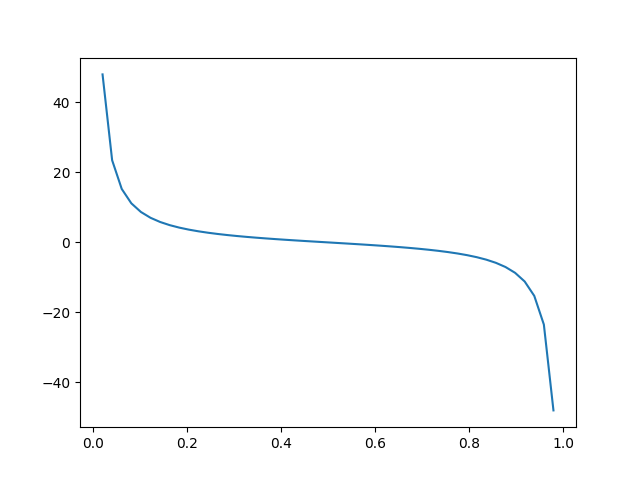
\includegraphics[scale=0.5]{functionofs.png}
\caption{Function $\frac{1}{x}+\frac{1}{x-1}$ on $[0;1]$}
\label{fig:functionofs}
\end{figure}

This function tends respectively to $\infty$ and $-\infty$ in $0$ and $1$ and is $0$ in $\frac{1}{2}$.
The second part of the function, $s(1-s)$, is added to ensure that $s$ stay in $[0;1]$.
This is proved by the two following theorems. \\

\begin{theorem}{}
The vector field $f$ of system (\ref{eq:1dsimple}) together with (\ref{eq:sdyn1}) is Lipschitz continuous on $A = [\gamma, 1-\gamma] \times [0;1]$
\end{theorem}

\begin{proof}
Let's denote by $\{ a_{ii}\}$ the components of the Jacobian of $f$.
We have
\begin{equation}
\label{eq:jacob}
\begin{cases}
a_{11} = sax^{a-1} - s(a+1)x^a - (1-s)(1-s)^a + a(1-s)(1-x)^{a-1} \\
a_{12} = (1-x)^a + x(1-x)^a \\
a_{21} = (-\frac{1}{x^2}-\frac{1}{(x-1)^2})s(1-s) \\
a_{22} = (\frac{1}{x}+\frac{1}{x-1})(1-2s) \\
\end{cases}
\end{equation}
As all the components are bounded in $A$, the vector field is Lipshitz continuous.
\end{proof}

\begin{theorem}{}
\label{posinv}
If $S$ is given by equation (\ref{eq:sdyn1}) and if $a>0$, then the set $A = [\gamma, 1-\gamma] \times [0;1]$ for any $\gamma > 0$ is positively invariant for system (\ref{eq:1dsimple}).
\end{theorem}

\begin{proof}
We will first show that there exists four particular trajectories that correspond respectively to the four side of the square A, i.e. the side $x=\epsilon$, $x=1-\epsilon$, $s=0$ and $s=1$. \\
For $x=0$, as the interval on $x$ is open, we will show that we have a trajectory as close as we want to the side of the square.
Let $\epsilon_1>0$ and $\epsilon_2 >0$, there exists $\delta > 0$ and $T > 0$ such that if $x < \delta$ and  if $\epsilon_1>s_0>0$, $s(t) > 1- \epsilon_2 \, \, \forall t > T$.
Indeed, if $x = \delta$ and  if $s=\epsilon_1$, the system becomes
\[
\begin{cases}
\dx =  (1-\delta)\epsilon_1\delta^a - \delta (1-\epsilon_1) (1-\delta)^a  \\
\ds = (\frac{1}{\delta}+\frac{1}{\delta-1})(1-\epsilon_1)\epsilon_1 \\
\end{cases}
\]
Therefore, we have that $\underset{\delta \rightarrow 0}{\text{lim}} \dx = 0$, $\underset{\delta \rightarrow 0}{\text{lim}} \ds = \infty$ wich means that $s$ will become enventually as close as we want to $1$. By symmetry, we can use a similar argument for the side $x=1$.
When $s=0$, $\ds = 0$ and $\dx = -x(1-x)^a < 0 \, \forall{x}$ so that $x$ decreses from $1-\epsilon$ to $\epsilon$ for each $\epsilon$ and similarly for $s=1$.
This shows that there exists four particular trajectories that correspond respectively to the four sides of the square A.
Now, as the vector field is Lipshitz continuous on $A$, the existence and unicity of solutions holds.
This means that trajectories cannot cross.
Therefore, each trajectory that will start inside $A$, will stay in $A$.
\end{proof}

The system has only one equilibirum point inside $A$, the point $(\frac{1}{2}, \frac{1}{2})$.
If both language have the same status and the same number of speakers, then no language will extinct and the system will stay as such forever.
We suppose that this fixed point is unstable.
Let us verify this mathematically.
The Jacobian matrix $\mathcal{A}$ was given by equation (\ref{eq:jacob}).
If we compute the eigenvalues of $\mathcal{A}$ at $(\frac{1}{2}, \frac{1}{2})$ for $a=1.31$, we have indeed that
\[
\begin{cases}
\lambda_1 = 0.194602+1.08263i \\
\lambda_2 = 0.194602-1.08263i \\
\end{cases}
\]
As the real part of both eigenvalues are positive, the equilibrium is unstable. \\
We will now show that the system evolves towards a limit cycle or a closed orbit by using Poincarré-Bendixson theorem.
Let us recall this theorem. \\

\begin{theorem}{Poincarré-Bendixson}
\label{th:pb}
Let $\dx = f(x)$ be a dynamical system with $x \in \mathbb{R}^2$. Let $R$ be a closed bounded subset of $\mathbb{R}^2$ that contains no equilibrium points. Let $t\rightarrow x(t)$ be a trajectory that stays in $R$ for all $t > 0$ and suppose that $f \in C^1$ in an open subset that contains $R$.\\
Then, $x(t)$ is a periodic solution or $x(t)$ tends towards a closed orbit ad $t \rightarrow \infty$.
\end{theorem}

To apply this thoerem to our system, let $\epsilon > 0$ and let $R = A \backslash B(\epsilon;(\frac{1}{2},\frac{1}{2}))$. We have shown that $(\frac{1}{2},\frac{1}{2})$ is unstable and $A$ is positively invariant. Therefore, all trajectories satisfy the assumptions of theorem \ref{th:pb}. \\

To end this part, here are some simulations of trajectories that can be observed for this system (Figure \ref{fig:traj1D1}) :

\begin{figure}[H]
\centering
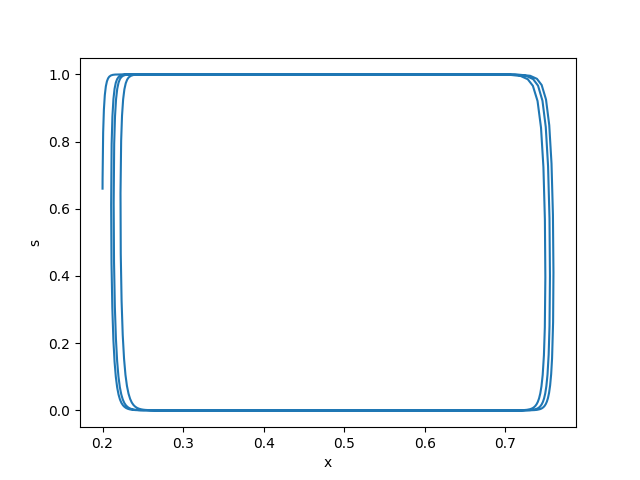
\includegraphics[scale=0.5]{traj1D1_02066.png}
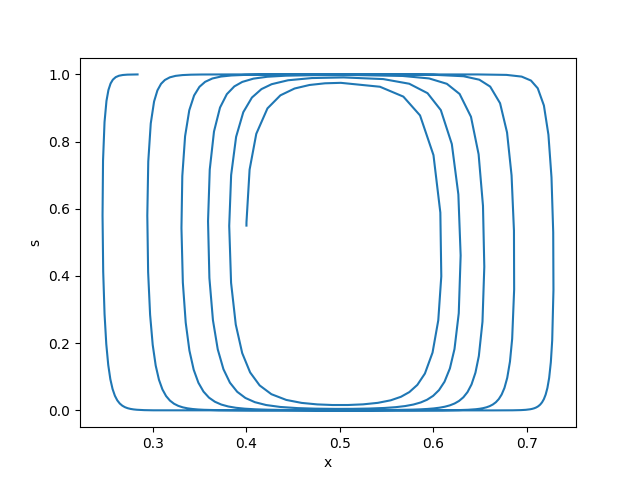
\includegraphics[scale=0.5]{traj1D1_04055.png}
\caption{Trajectories for the system \ref{eq:1dtemp} with status dynamic \ref{eq:sdyn1}. Starting points are respectively $[x_0, s_0] = [0.2, 0.66] \text{   and   } [0.4, 0.55]$.}
\label{fig:traj1D1}
\end{figure}

We can see that indeed the trajectories seem to converge to a periodic trajectory.

\subsection*{Alternative status dynamic}
The addition of a dynamical model for the status makes it possible to explain why some languages, although previously endangered and close to extinction, experience a renewed status and a change in dynamics.
This is for instance the example of the Irish languange and the Walloon language.
However, this system doesn't explain extinction as it is impossible with that dynamic.
It is possible to slightly modify the dynamic and come up with a system that will have both possibilities of extinction and of renewed popularity, closer to what seems to happen in the real world.
This is done by modifying the $S(x,s)$ function to remove the asymptotic behavior in $0$ and $1$.
I propose the following dynamic for $s$ :

\begin{equation}
\label{eq:sdyn2}
S(x,s) =  \alpha (\frac{1}{x+1} + \frac{1}{x-2}) (1-s) s
\end{equation}

where $\alpha \in \mathbb{R}_{+}$ is a nonnegative parameter. If, similarly to Figure \ref{fig:functionofs}, we plot the first factor of $S(x,s)$ as a funciton of $s$, we have

\begin{figure}[H]
\centering
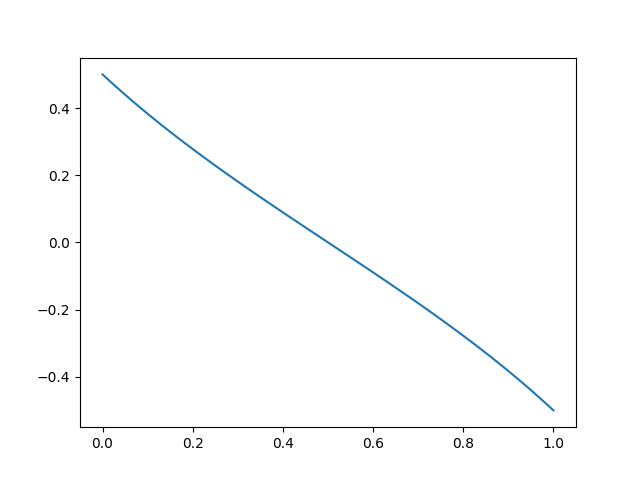
\includegraphics[scale=0.5]{functionofs2.png}
\caption{Function $\frac{1}{x+1}+\frac{1}{x-2}$ on $[0;1]$}
\label{fig:functionofs2}
\end{figure}

This function ensures that the language close to extinction will indeed benefit from a renewed popularity, but the popularity will be limited.
The strength of this renewal is controlled by parameter $\alpha$. \\
Intuitively, we would think that this new dynamic doesn't prevent a language to extinct like the previous one.
Indeed, this is what we observe.
For example, Figure \ref{fig:traj1D2} shows some of the possible trajectories for this system.

\begin{figure}
\centering
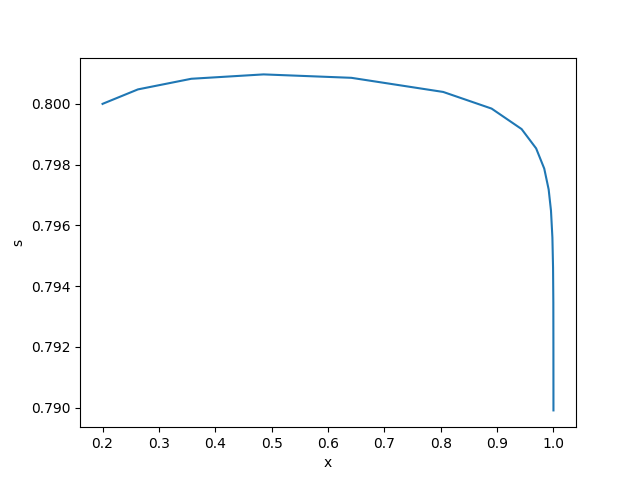
\includegraphics[scale=0.4]{traj1D202081e-3.png}
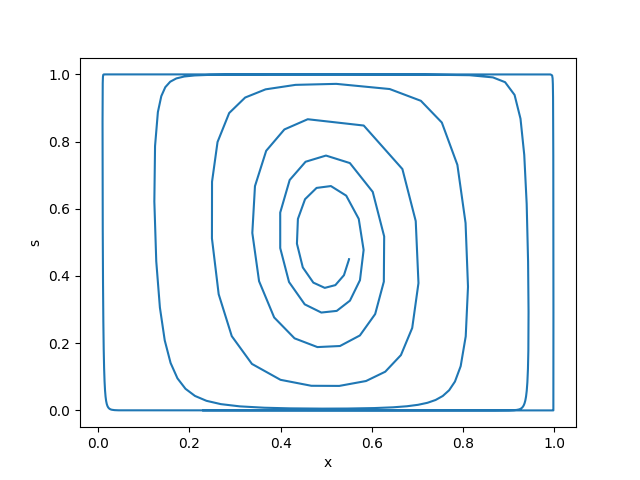
\includegraphics[scale=0.4]{traj1D20550451.png}
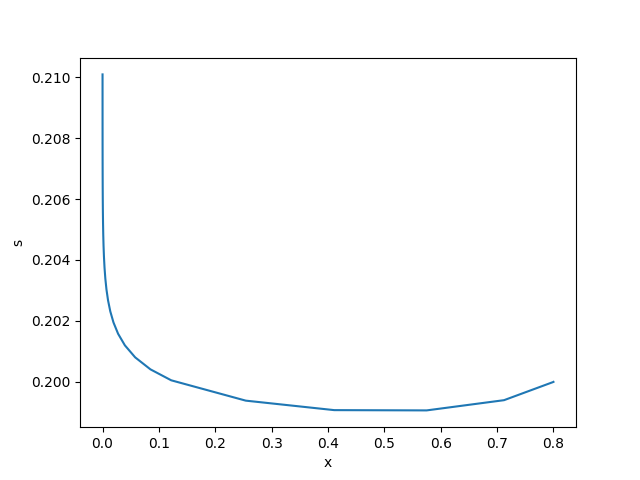
\includegraphics[scale=0.4]{traj1D208021e-3.png}
\caption{Trajectories for the system \ref{eq:1dtemp} with status dynamic \ref{eq:sdyn2}. Starting points are respectively $[x_0, s_0] = [0.2, 0.8], [0.55,0.55] \text{   and   } [0.4, 0.55]$. The value of $\alpha$ is respectively $10^{-3}$, $1$ and $10^{-3}$.}
\label{fig:traj1D2}
\end{figure}

This shows that indeed, if $\alpha$ remains small, it is possible for a language to extinct.
If $\alpha$ is somehow large like for the central plot, what seems to be a periodic solution is observed, similarly than for the previous $S$.\\
Simlarly to theorem \ref{posinv}, we can show that the dynamic is well defined. \\
\begin{theorem}{}
\label{posinv2}
If $S$ is given by equation (\ref{eq:sdyn2}) and if $a>0$, then the set $B = [0;1] \times [0;1]$ is positive invariant for system (\ref{eq:bil}).
\end{theorem}

\begin{proof}
Similarly than for theorem \ref{posinv}, we will show that the four sides of B are trajectories. \\
If $s = 0$ and $x_0 = 1-\epsilon$, then $\ds = 0$ and $\dx < 0$. Therefore $x$ will decrese until $0$.
We thus have that the side $s=0$ is a trajectory.
By symmetry, $s=1$ is a trajectory.
If $x=0$ then $\dx = 0$. If in addition, $s_0 = 1-\epsilon$, $\ds < 0$ for all $s < 1$ and it will decrease until $0$.
By symmetry, the sides $x=0$ and $x=1$ are trajectories.
This shows by a similar argument than the one used in theorem \ref{posinv} that  B is positively invariant.
\end{proof}

Let us now analyse more formally the fixed points of this systems.
The nullclines are
$$n_x = \{(x,s) | x=0 \} \cup \{ (x,s)| x = 1 \} \cup \{ (x,s) | sx^{a-1} = (1-s)(1-x)^{a-1} \}$$
$$n_s = \{(x,s) | s=0 \} \cup \{ (x,s)| s = 1 \} \cup \{ (x,s) | x= \frac{1}{2} \}$$

Taking the intersection of the nullclines, we get that the fixed point of this system are the four vertices of $B$ anf $(\frac{1}{2}, \frac{1}{2})$.
Now let us look at their stability.
We consider only the case $a=1.31$ for simplicity.
Similarly than for the previous system, we get the following components for the jacobian

\[
\begin{cases}
a_{11} = sax^{a-1} - s(a+1)x^a - (1-s)(1-s)^a + a(1-s)(1-x)^{a-1} \\
a_{12} = (1-x)^a + x(1-x)^a \\
a_{21} = (-\frac{1}{(x+1)^2}-\frac{1}{(x-2)^2})s(1-s) \\
a_{22} = (\frac{1}{x+1}+\frac{1}{x-2})(1-2s) \\
\end{cases}
\]

The eigenvalues can then be conputed for each of the fixed points given above.
We have
\begin{table}[h]
  \centering
  \begin{tabular}{cccccc}
    & $(0,0)$ & $(1,0)$ & $(1,0)$ & $(1,1)$ & $(\frac{1}{2}, \frac{1}{2})$ \\
    \hline
    $\lambda_1$ & 0.31 & -1 & 0 & -1 & $0.194602+0.310758i$ \\
    \hline
    $\lambda_2$ & 0.5 & -0.5 & -0.5 & 0.5 & $0.194602-0.310758i$ \\
    \hline
  \end{tabular}
  \caption{Eigenvalues of system \ref{eq:1dtemp} for $a=1.31$.}
  \label{tab:eig}
\end{table}

We have that $(0,0), (1,1)$ and $(\frac{1}{2}, \frac{1}{2})$ are unstable. $(1,0)$ is stable and the stability of $(0,1)$ is undetermined with this linear analysis.
These results are consistent with Figure \ref{fig:traj1D2} which shows two trajectories converging respectively to $(0,1)$ and $(1,0)$.
This figure also suggest that the basin of attraction of these stable fixed points depend on $\alpha$ and on the intial $s$.
Intuitively, the smaller the value of $\alpha$ and the larger the intial status, the more chances we have to see the extinction of language $Y$.
Conversely, the smaller the value of $\alpha$ and the smaller the intial status, the more chances we have to see the extinction of laguage $X$.
To confirm this, I simulated the long term behavior of the system with respect to $\alpha$ and $s_0$.
The following heat map (Figure \ref{fig:heatmap}) shows the results :

\begin{figure}[H]
\centering
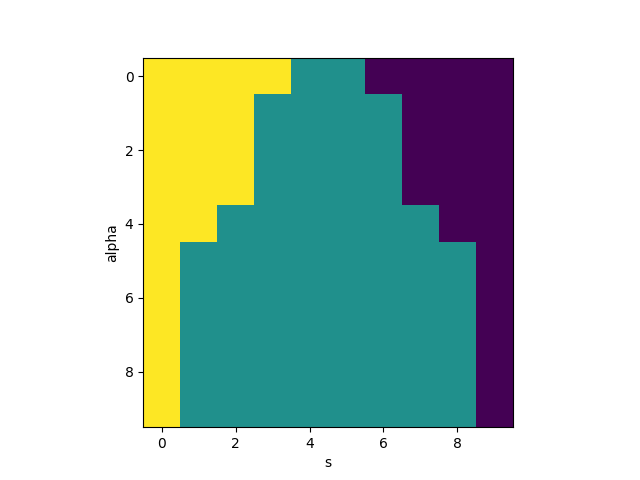
\includegraphics[scale=0.5]{convergence_heatmap.png}
\caption{Heat map of the long term behavior of the system with respect to the initial status and the parameter $\alpha$. In yellow, the trajectories that converged to $(0,1)$. In purple, the trajectories that converged to $(1,0)$. In blue, the trajectories that did not converged to any of the fixed point.}
\label{fig:heatmap}
\end{figure}

This map confirms our intuition and shows the symmetric pattern around $s=\frac{1}{2}$.

\section{Temporal extension for model with bilinguism}
\label{sec:2d}
As discussed in section \ref{sec:basic}, people came up with extensions to the system \ref{eq:1dsimple} to take into account the important notion of bilinguism.
In \cite{bilingual}, system \ref{eq:bil} is presented.
Using notations described previously this system follows the evolution of the proportion of $X$ speakers, $Y$ speakers and bilinguals, respectively $x$, $y$ and $b$.
These proportions, by definition, are linked by the equation $x+y+b = 1$.
System \ref{eq:bil} is thus actually a 2D system.
We can extend our language status dyamic in a straightforward way and write the following 3D system :

\begin{equation}
\label{eq:2d}
\begin{cases}
\dx = c(1-x) \Big( (1-k)s(1-y)^a - (1-s)x(1-x)^{a-1} \Big) \\
\dy = c(1-y) \Big( (1-k)(1-s)(1-x)^a - sy(1-y)^{a-1} \Big) \\
\ds = \alpha \Big( \frac{1}{x+1} - \frac{1}{y+1}\Big) s (1-s) \\
\end{cases}
\end{equation}

We restrict here without loss of generality to the case $c=1$.
Let us see if coexistence is still possible with this dynamics in $s$.
The nullcline of $s$ can be written as

$$n_s = \{(x,y,s) | x = y \} \cup \{(x,y,s)| s = 0\} \cup \{(x,y,s) | s = 1\}$$

The point $s=0$ and $s=1$ will correspond to the fixed points located at the border of the domain.
The interesting case happens when $x=y$.
In this case, the nullclines are symmetrical w.r.t. the line $x=y$.
Adding the nullcline corresponding to $s$, Figure 2 of \cite{bilingual} becomes

\begin{figure}[H]
\centering
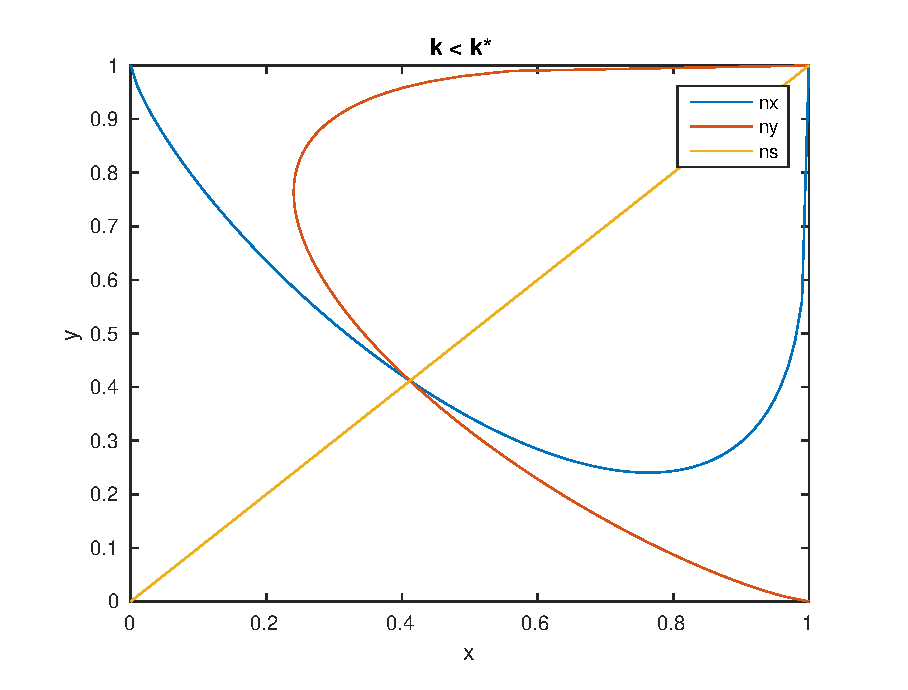
\includegraphics[scale=0.5]{nullpp.eps}
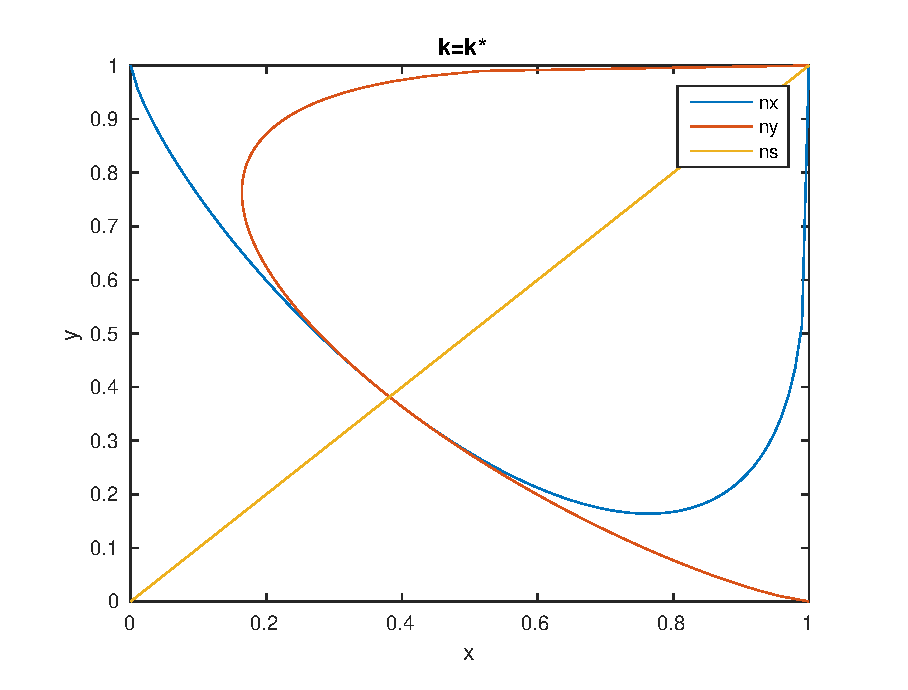
\includegraphics[scale=0.5]{nulle.eps}
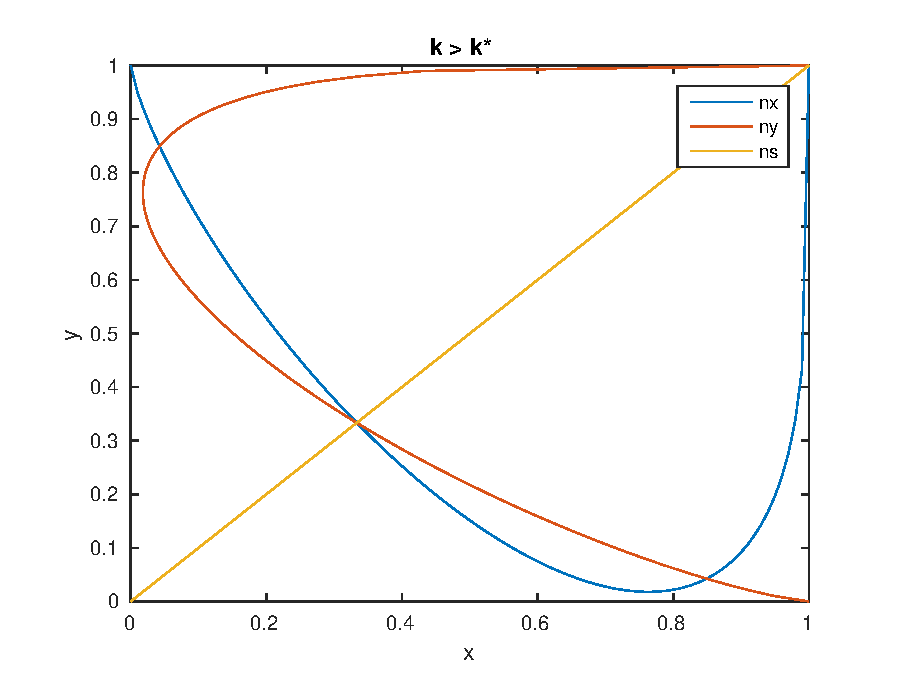
\includegraphics[scale=0.5]{nullpg.eps}
\caption{Nullclines of the system in the plane $s=\frac{1}{2}$}
\label{fig:nullclines}
\end{figure}

The equilibria correponds to the intersection of the nullclines.
Therefore, we have one equilibrium located in $(\frac{1-k}{2-k}, \frac{1-k}{2-k}, \frac{1}{2})$.
This equilibrium was thoroughly studied in \cite{bilingual}.
On Figure \ref{fig:nullclines}, we can see that at $k=k^{\ast}$, two equilibria appears for the system with constant $s$.
This suggests a Pitchfork bifurcation and it is indeed the case as shown in the paper.
The result is then extended to the more general case where $s \ne \frac{1}{2}$.
The bifurcation parameter was obtained as a function of $s$.
The region where this equilibrium is stable is represented in the following figure (Figure \ref{fig:coexistence})

\begin{figure}[H]
\centering
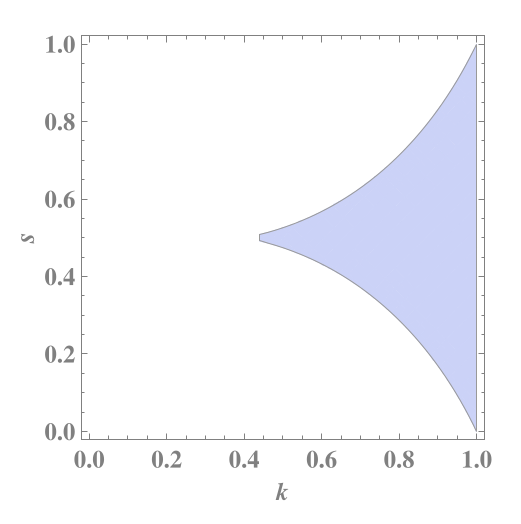
\includegraphics[scale=0.5]{coexistence.png}
\caption{Coexistence region in function of $s$ and $k$. Source : \cite{bilingual}}
\label{fig:coexistence}
\end{figure}

What about the stability of our equilibrium ?
The bifurcation analysis of \cite{bilingual} suggests also a change of stability at $k=k^{\ast}$.
Indeed, for $k<k^{\ast}$, the equilibrium was shown to be unstable and the addition of a dynamic in $s$ won't stabilize it.
For $k>k^{\ast}$ however, the equilibrium was shown to be stable in the 2D system.
On figure \ref{fig:coexistence}, we see that perturbating slightly $s$ leaves the system in its stability region and we would thus guess that $s$ doesn't perturb the stability.
This is of course not a rigorous analysis.
To be further convinced that there is indeed a change of stability for our system at $k=k^{\ast}$, we can compute numerically the eigenvalues of the Jacobian and check their sign.
Figure \ref{fig:bifur} shows what we obtain.

\begin{figure}[H]
\centering
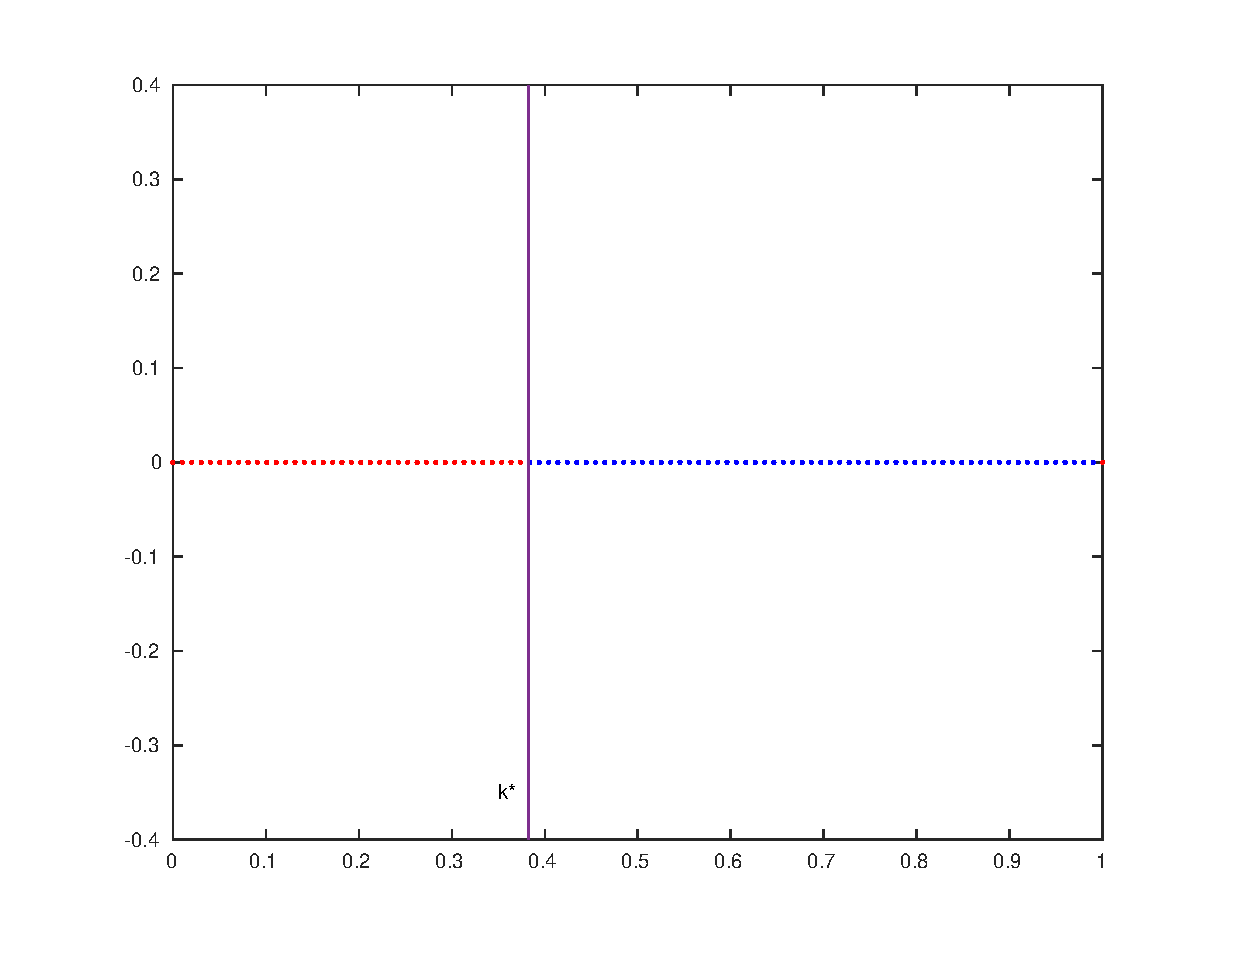
\includegraphics[scale=0.5]{bifur.eps}
\caption{Numerical simulation of the stability of the equilibrium for system \ref{eq:2d}. Red corresponds to unstability while blue corresponds to stability. The vertical line represent $k=k^{\ast}$.}
\label{fig:bifur}
\end{figure}

This simulation confirms the change in stability at $k=k^{\ast}$.

\section{Spatial analysis}
\label{sec:spatial}
When Abrams and Strogatz first proposed a model for the language dynamics in \cite{death}, they claimed that the evolution was driven by the number of speakers in both language and the perceived status of the language among the population.
The status was considered constant throughout the time.
The analysis provided in the previous sections studied the dynamics of language when we relax this strong constraint. \\
Another implicit strong constraint in the model is the spatial uniformity of the dynamics.
If it is true that the dynamic is driven by the number of speakers, it suggests that we are somehow influenced by the part of the population that speaks the other language.
In this context, it seems natural that we will be much more influenced by our neighbors than by people living far away. \\
To illustrate this, I will agin take the example of the Irish language.
Although the proportion of Irish speakers is quite low at the scale of the whole country, there are regions where this proportion is much higher than the average (in this case, mainly in county Galway and Mayo in the West part).
The people living in these regions would be influenced by the proportion of speakers in their own region and not by the average over the country.\\
To study this phenomenon, let's go back to the simplest model from Abrams and Strogatz.
Instead of considering one state variable for the whole country, let's divide the country into $K$ regions of similar surface.
We add one state variable $x_k$ per region, corresponding to the proportion of speakers of language $X$ in region $k \in \{ 1, ..., K\}$.
We define the neighbors of a region $k$ as the set of regions that have a nonpunctual border with it and we denote by $\mathcal{N}_k(x)$ the mean of the state variables of the neighbors of $k$.
The spatial evolution of the number of speakers can be modeled as

\begin{equation}
\dx_k = c\big( (1-x_k)s\mathcal{N}(x)^a - x_k(1-s)(1-\mathcal{N}(x))^a \big) \hspace{1cm} \forall k \in \{1,...,K\}
\end{equation}

This model was tested on a real Irish dataset.
In this dataset, each region correspond to one electoral district.
We considered a square grid, changing slightly the shape of the country but trying as much as possible to keep the neighbor relationship as such.
The following figure (Figure \ref{fig:firstandlast_ir}) represent the first and last frame of the simulation

\begin{figure}[H]
\centering
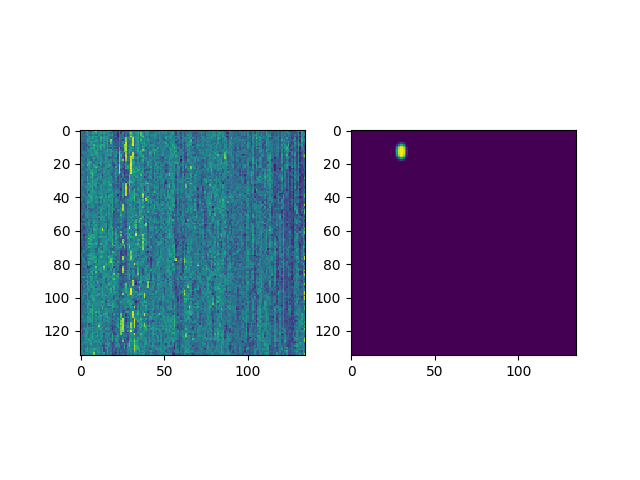
\includegraphics[scale=0.5]{firstandlast_ir.png}
\caption{First and last frame of the simulation of the spatial model on the Irish dataset. Yellow corresponds to only Irish speakers while purple represents only English speakers. It was obtained for $s=\frac{1}{2}$}
\label{fig:firstandlast_ir}
\end{figure}

The region that were surrounded by a majority of English speakers become quickly English speaking only.
It is true for Irish, too.
This is due to how Abrams and Strogatz's model behave, preventing coexistence.
Let's compare the two overall dynamics.
The following figure (Figure \ref{fig:overall}) represent the average of Irish speakers in Ireland using both models

\begin{figure}[H]
\centering
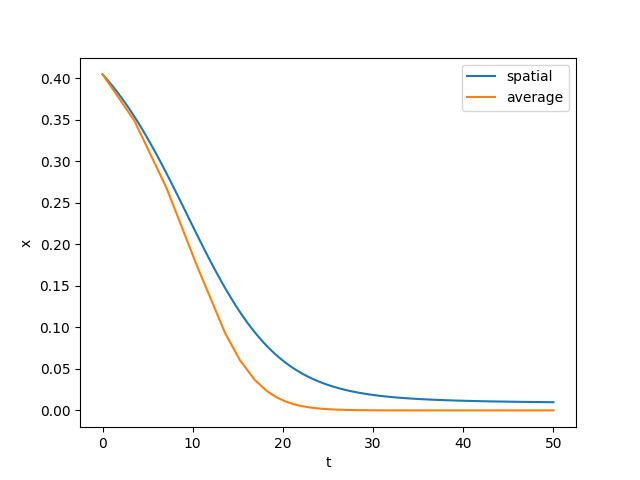
\includegraphics[scale=0.5]{overall_dyn_ir.png}
\caption{First and last frame of the simulation of the spatial model on the Irish dataset. Yellow corresponds to only Irish speakers while purple represents only English speakers. It was obtained for $s=\frac{1}{2}$}
\label{fig:overall}
\end{figure}

This shows, as we would intuitively expect, that the spatial dynamic is slower than the average dynamic over the country.
Therefore, one should be careful when interpreting the results of the models.
If the time scale is important in the analysis, adding a spatial dependence, similarly than what was presented here, would probably give more accurate results.

\newpage
\section{Conclusion}
\label{sec:conclusion}
Half of the languages on this planet are directly endangered and the rate at which the extinction occurs is alarming.
To come up with suitable policies for the preservation of these languages, a theoretical analysis from the point of view of dynamical systems can be very helpful. \\
In this work, we first described the basic systems that are commonly used to model language dynamics.
Then, we proposed mainly two extensions to these models to take into account temporal and spatial evolutions of the parameters.
Some theoretical results were obtined and numerical simulations were conducted. \\
The analysis performed in this project shows that adding both a dynamic status and spatial considerations modify sometimes significantly the behavior of the systems. \\
This project aimed to give a first picture of what a temporal and spatial analysis of language dynamics could look like but the goal was not to be comprehensive. In particular, the intuition was often given using numerical simulations. In a further work, it could be interesting to derive more theoretical results to prove rigorously what was obtained. Moreover, testing the models on real datasets and possibly adapting in consequence the models proposed would probably be the next step for this work.


\bibliographystyle{plain}
\bibliography{references}

\end{document}
